%------------------------------------------------------------------------------
% Author(s):
% Varaun Ramgoolie
%
% Copyright:
%  Copyright (C) 2020 Brad Bachu, Arjun Mohammed, Varaun Ramgoolie, Nicholas Sammy
%
%  This file is part of Applied-Mathematics-Unit2 and is distributed under the
%  terms of the MIT License. See the LICENSE file for details.
%
%  Description:
%     Year: 2013
%     Module: 3
%     Question: 6
%------------------------------------------------------------------------------

%------------------------------------------------------------------------------
% 6 a
%------------------------------------------------------------------------------

\begin{subquestions}
	
\subquestion

We are given two masses which are connected by a string over a smooth, weightless pulley.

\begin{subsubquestions}
	
\subsubquestion

\textbf{\textit{Sketch and Translate:}} \\ \\
\begin{figure}[H]
	\begin{center}
		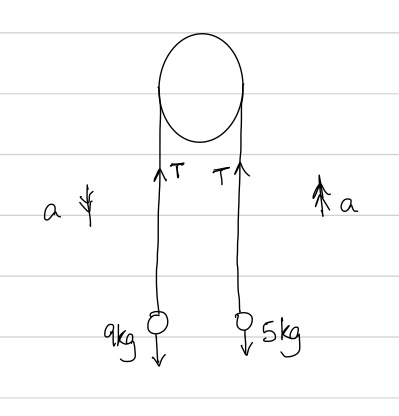
\includegraphics[scale=0.25]{../2013/figures/2013q6-1}
		\caption{\label{2013:q6:Sketch1} Pulley System.}
	\end{center}
\end{figure}	
We are asked to find the acceleration of the system given. This problem is a classic pulley problem and so, we should think about what we know about tension and forces in the context of pulleys.




\textbf{\textit{Simplify and Diagram:}} \\ \\
\begin{figure}[H]
	\begin{center}
		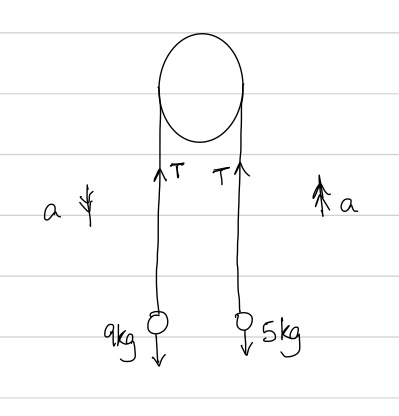
\includegraphics[scale=0.25]{../2013/figures/2013q6-1}
		\caption{\label{2013:q6:Diagram1} All forces on Pulley System.}
	\end{center}
\end{figure}
We will assume that both bodies move in only 1 dimension and that they behave as point particles. We will also assume that the mass of the string is 0 and inextensible. Thus, we know that the speed (and the magnitude of the acceleration) of both particles must be the same. Since the pulley is smooth, no energy is lost to friction. We should consider how the forces act on the different weights and motivate our solution from there.
We will define the following:
\begin{itemize}
	\item $\vec{W_1}$ is the weight of the 9kg mass,
	\item $\vec{W_2}$ is the weight of the 5kg mass,
	\item $\vec{T_1}$ is the tension on the string from the 9kg mass to the pulley,
	\item $\vec{T_2}$ is the tension on the string from the 5kg mass to the pulley,
	\item $m_1$ is the mass of the 9kg mass, $m_1=9$,
	\item $m_2$ is the mass of the 5kg mass, $m_2=5$.
\end{itemize}



\textbf{\textit{Represent Mathematically:}} \\ \\ 
Let us denote the displacements of the 9kg and 5kg masses so be $y_1$ and $y_2$. As the string is inextensible, we know that,
\begin{align}
	y_1 & = -y_2 \nn \\
	\implies \ddd{y_1}{t} & = -\ddd{y_2}{t} \nn \\
	\implies \ddd{^2y_1}{t^2} & = -\ddd{^2y_2}{t^2} \nn \\
	a_1 & = -a_2 \,.
\end{align}

From the assumption that the string is massless, we also get that,
\begin{equation}
	|\vec{T_1}| = |\vec{T_2}| = T \,.
\end{equation}

Let us now consider the forces on the 9kg mass. From Newton's 2nd Law, we get that,
\begin{align}
	\sum F & = m_1a_1 \nn \\
	|\vec{W_1}| - T & = m_1a_1 \,.
\end{align}

Let us then consider the forces on the 5kg mass. From Newton's 2nd Law, we get that,
\begin{align}
	\sum F & = m_2a_2 \nn \\
	|\vec{W_2}|-T & = m_2a_2 \,.
\end{align}




\textbf{\textit{Solve and Evaluate:}} \\ \\
On the 9kg mass, we see that,
\begin{align}
	m_1g - T & = m_1a_1 \nn \\
	\implies 9g-T & = 9a_1 \,. \label{2013:q6:PulleyEq1}
\end{align}

On the 5kg mass, we see that,
\begin{align}
	m_2g - T & = m_2a_2 \nn \\
	\implies 5g-T & = 5a_2 \nn \\
	\implies 5g-T & = -5a_1 \nn \\
	T-5g & = 5a_1 \,. \label{2013:q6:PulleyEq2}
\end{align}

By solving \req{2013:q6:PulleyEq1} and \req{2013:q6:PulleyEq2} simultaneously, we get,
\begin{align}
	\text{(\req{2013:q6:PulleyEq1}+\req{2013:q6:PulleyEq2}):} (9g-T)+[T-5g] & = (9a_1)+[5a_1] \nn \\
	4g & = 14a_1 \nn \\
	\implies a_1 & = a = \frac{4}{14}g = 2.86\text{ms}^{-2} \,.
\end{align}

%------------------------------------------------------------------------------

\subsubquestion

\textbf{\textit{Solve and Evaluate:}} \\ \\
We can find the tension on the string by substituting our value from (a)(i) into \req{2013:q6:PulleyEq2}. We get,
\begin{align}
	T-5g & = 5a_1 \nn \\
	T & = 5a_1 + 5g \nn \\
	  & = 5\left(\frac{4}{14}g \right) + 5g \nn \\
	  & = \frac{90}{14}g = 64.29N \,.
\end{align}

%------------------------------------------------------------------------------

\subsubquestion

\textbf{\textit{Simplify and Diagram:}} \\ \\
We can use consider \rfig{2013:q6:Diagram1}. We will assume that our particles were released from rest. As we have the acceleration of our particles, we can use our equations of motion and solve for the displacement of the particle(s).




\textbf{\textit{Represent Mathematically:}} \\ \\
We can consider either particle. As we have taken the downwards direction to be positive, we will consider the 9kg mass. We can find the displacement of the particle using,
\begin{equation}
	s=ut+\frac{1}{2}at^2 \,.
\end{equation}




\textbf{\textit{Solve and Evaluate:}} \\ \\
By substituting $u=0\text{ms}^{-1}$, $t=6$s and $a=2.86\text{ms}^{-2}$, we can find that,
\begin{align}
	s & = ut+\frac{1}{2}at^2 \nn \\
	  & = (0)(6) + \frac{1}{2}(2.86)(6)^2 \nn \\
	  & = 51.48m \,.
\end{align}

\end{subsubquestions}

%------------------------------------------------------------------------------
% 6 b
%------------------------------------------------------------------------------

\subquestion

\textbf{\textit{Sketch and Translate:}} \\ \\
\begin{figure}[H]
	\begin{center}
		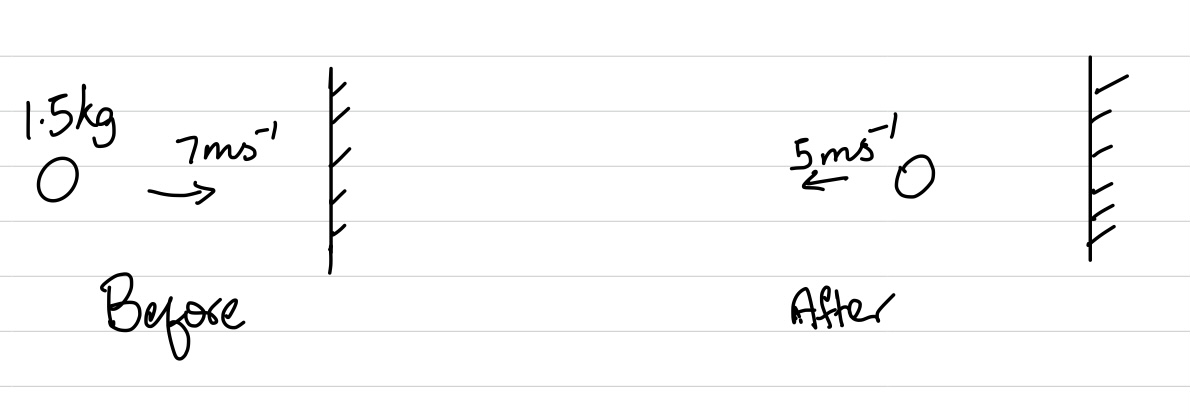
\includegraphics[scale=0.25]{../2013/figures/2013q6-2}
		\caption{\label{2013:q6:Sketch2} Ball hitting wall.}
	\end{center}
\end{figure}	
We are given a ball which strikes a wall and bounces back. We should think about what we know about impulse and how impulse is related to the velocities of the ball.




\textbf{\textit{Simplify and Diagram:}} \\ \\
\begin{figure}[H]
	\begin{center}
		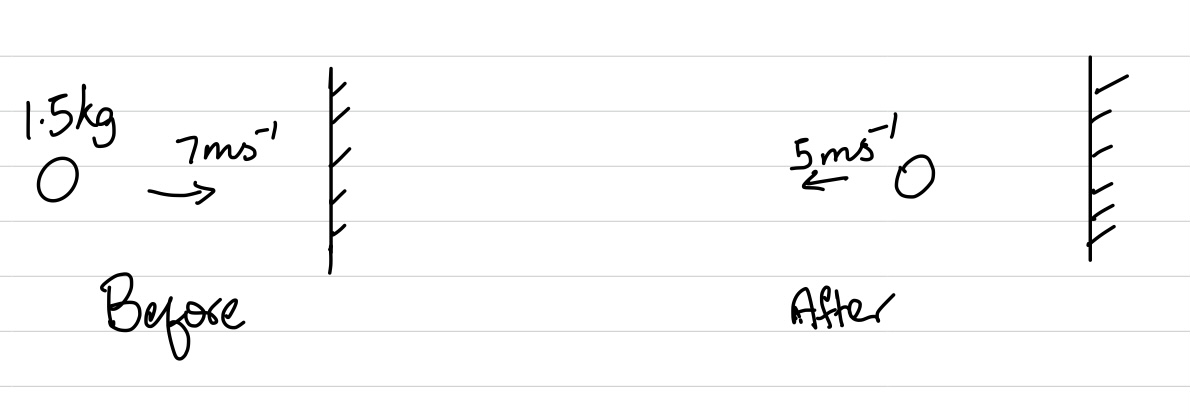
\includegraphics[scale=0.25]{../2013/figures/2013q6-2}
		\caption{\label{2013:q6:Diagram2} Ball hitting and bouncing back from wall.}
	\end{center}
\end{figure}	
We will assume that the body only moves in one plane (horizontal). We will take the direction of the rebound of the ball as positive. We can use our equation for impulse and solve this question.
We will define the following:
\begin{itemize}
	\item $m$ is the mass of the ball, $m=1.5kg$,
	\item $u$ is the initial velocity, $u=-7\text{ms}^{-1}$,
	\item $v$ is the final velocity, $v=5\text{ms}^{-1}$.
\end{itemize}




\textbf{\textit{Represent Mathematically:}} \\ \\
By definition, we know that,
\begin{align}
	\text{Impulse} & = \text{Final Momentum} - \text{Initial Momentum} \nn \\ 
	               & = mv - mu \,.
\end{align}




\textbf{\textit{Solve and Evaluate:}} \\ \\
By substituting our values, we get,
\begin{align}
	\text{Impulse} & = mv-mu \nn \\
	               & = 1.5(5-(-7)) \nn \\
	               & = 18Ns \,.
\end{align}

%------------------------------------------------------------------------------
% 6 c
%------------------------------------------------------------------------------

\subquestion

\textbf{\textit{Simplify and Diagram:}} \\ \\
\begin{figure}[H]
	\begin{center}
		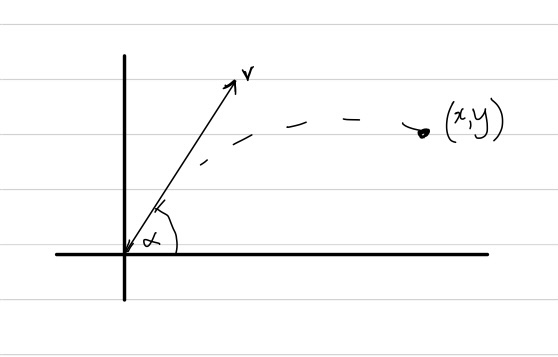
\includegraphics[scale=0.25]{../2013/figures/2013q6-3}
		\caption{\label{2013:q6:Diagram3} Motion of Projectile.}
	\end{center}
\end{figure}
We want to describe the trajectory of a projectile with an equation. We can do this by considering the vertical and horizontal motion of the projectile separately and linking both using the time variable, $t$. We will use,
\begin{itemize}
	\item $\vec{v}$ to represent the initial velocity of the particle,
	\item $\alpha$ to represent the angle of projection to the horizontal,
	\item $y$ to represent the vertical displacement of the particle,
	\item $x$ to represent the horizontal displacement of the particle,
	\item $u_x$ to represent the initial velocity of the particle in the horizontal ($x$) direction,
	\item $u_y$ to represent the initial velocity of the particle in the vertical ($y$) direction,
	\item $a_x$ tp represent the acceleration in the $x$ direction,
	\item $a_y$ to represent the acceleration in the $y$ direction,
\end{itemize}  




\textbf{\textit{Represent Mathematically:}} \\ \\
Firstly, we should notice that we can resolve $\vec{v}$ as\footnote{We will use the magnitude of $\vec{v}$ as $v$.},
\begin{equation}
	\vec{v} = v\cos(\alpha)\xhat + v\sin(\alpha)\yhat \,. \label{2013:q6:Eqn1}
\end{equation}

To complete the solution, we will use,
\begin{equation}
	s = ut + \frac{1}{2}at^2 \,.
\end{equation}




\textbf{\textit{Solve and Evaluate:}} \\ \\
From \req{2013:q6:Eqn1}, we get that.
\begin{align}
	v_x & = v\cos(\alpha) \\
	& \text{and} \nn \\
	v_y & = v\sin(\alpha) \,.
\end{align} 

We will first consider the horizontal motion of the particle. Using $a_x=0$,\footnote{There is no resistance to motion in the $x$ direction, which means that $a_x=0$} $s=x$ and $v_x=v\cos(\alpha)$, we get that,
\begin{align}
	s & = ut + \frac{1}{2}at^2 \nn \\
	x & = v\cos(\alpha)t + \frac{1}{2}(0)t^2 \nn \\
	\implies t & = \frac{x}{v\cos(\alpha)} \nn \\
	& = \frac{x\sec(\alpha)}{v} \,.
\end{align}	

We can now consider the vertical motion of the particle. Using $a_y=-g$,\footnote{The particle's acceleration in the $y$ direction is the acceleration due to gravity. The value is negative as we have taken up to be positive.} $s=y$, $v_y=v\sin(\alpha)$ and $t=\frac{x\sec(\alpha)}{v}$, we get that,
\begin{align}
	s & = ut + \frac{1}{2}at^2 \nn \\
	y & = v\sin(\alpha)\left(\frac{x\sec(\alpha)}{v}\right) + \frac{1}{2}(-g)\left(\frac{x\sec(\alpha)}{v}\right)^2 \nn \\
	& = x\tan(\alpha) - \frac{gx^2\sec^2(\alpha)}{2v^2} \,.
\end{align}

%------------------------------------------------------------------------------
% 6 d
%------------------------------------------------------------------------------

\subquestion

\textbf{\textit{Sketch and Translate:}} \\ \\
\begin{figure}[H]
	\begin{center}
		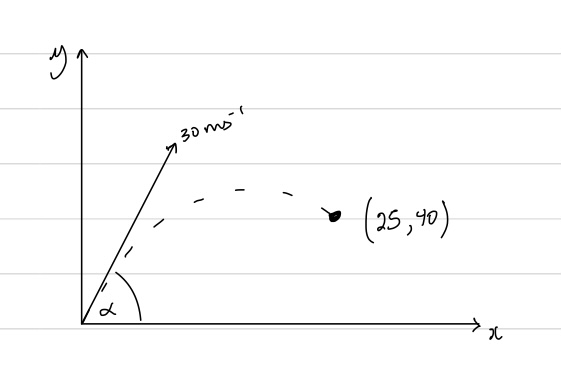
\includegraphics[scale=0.25]{../2013/figures/2013q6-4}
		\caption{\label{2013:q6:Sketch4} Motion of bullet.}
	\end{center}
\end{figure}
We want to find the possible angles at which the bullet was fired. As we have determined the equation of a projectile's trajectory, we should think about how we can use this to find values of $\alpha$. 




\textbf{\textit{Simplify and Diagram:}} \\ \\
\begin{figure}[H]
	\begin{center}
		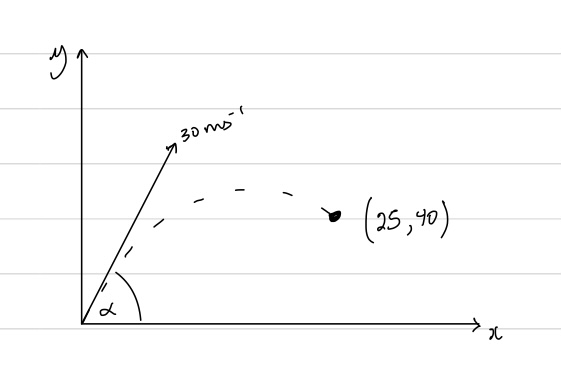
\includegraphics[scale=0.25]{../2013/figures/2013q6-4}
		\caption{\label{2013:q6:Diagram4} Motion of bullet.}
	\end{center}
\end{figure}
By using the information given in the question, we can substitute values into our equation and solve for $\alpha$.




\textbf{\textit{Represent Mathematically:}} \\ \\
We need to solve for $\alpha$ in the equation,
\begin{equation}
	y = x\tan(\alpha) - \frac{gx^2\sec^2(\alpha)}{2v^2}
\end{equation} 
    
    
    
    
\textbf{\textit{Solve and Evaluate:}} \\ \\
By substituting P(25,40) and $v=30$, we get that,
\begin{align}
	40 & = 25\tan(\alpha) - \frac{g(25)^2\sec^2(\alpha)}{2(30)^2} \nn \\
	 & = 25\tan(\alpha) - \frac{125\sec^2(\alpha)}{36} \nn \\
	 \implies 1440 & = 900\tan(\alpha) -125\sec^2(\alpha) \nn \\
	 1440 & = 900\tan(\alpha) -125(\tan^2(\alpha)+1) \nn \\
	 \implies 0 & = 125\tan^2(\alpha)-900\tan(\alpha) + 1565  \nn \\ 
\end{align}
  
By using the quadratic formula, we get that,
\begin{align}
	\tan(\alpha) & = \frac{900 \pm \sqrt{810000-782500}}{250} \nn \\
	             & = 3.6 \pm 0.66 \nn \\
	             \implies \alpha & = \arctan(4.26) = 77^o \nn \\
	             & \text{and} \nn \\
	             \alpha & = \arctan(2.94) = 71^o \,.
\end{align}


















	
\end{subquestions}